\begin{document}
	\chapter{Evaluation}
	\section{Success criteria} \label{Section: eval/success-criteria}
		blah
	\section{Features evaluation} \label{Section: eval/features}
		Even though the key module of the entire project was the one where the machine learning models are implemented, the set of features extracted for each node is at least as important because, without them being representative, the models will not be able to generalize well. For this reason, in this section, I will present the evaluation of the features I extracted for each node.
		
		\subsection{Feature ranking algorithm}
		Ranking the features selected is based on decision trees and is done using the \textbf{tree growing algorithm}. It is a greedy algorithm that observes the fact that the best splits are performing early while growing the decision tree. 
		
	\section{Evaluation of machine learning models} \label{Section: eval/ml}
	\subsection{Evaluation methodology} \label{Section: eval/ml/methodology}
		In order to quantitatively evaluate the performance of the machine learning models implemented, I used a labelled dataset $\mathbf{s}$ containing $5,498$ nodes. Figure \ref{Fig: eval/ml/methodology/dist} shows how the labels and node types are distributed in the dataset used in this case. From there, we can observe that the node type distribution resembles the distribution that can be found in the general case in a provenance graph. Therefore, by evaluating the models on this dataset I can produce a comprehensive and accurate assessment of their performance. 
		\begin{figure}[H]
			\centering
			\begin{subfigure}{.4\textwidth}
				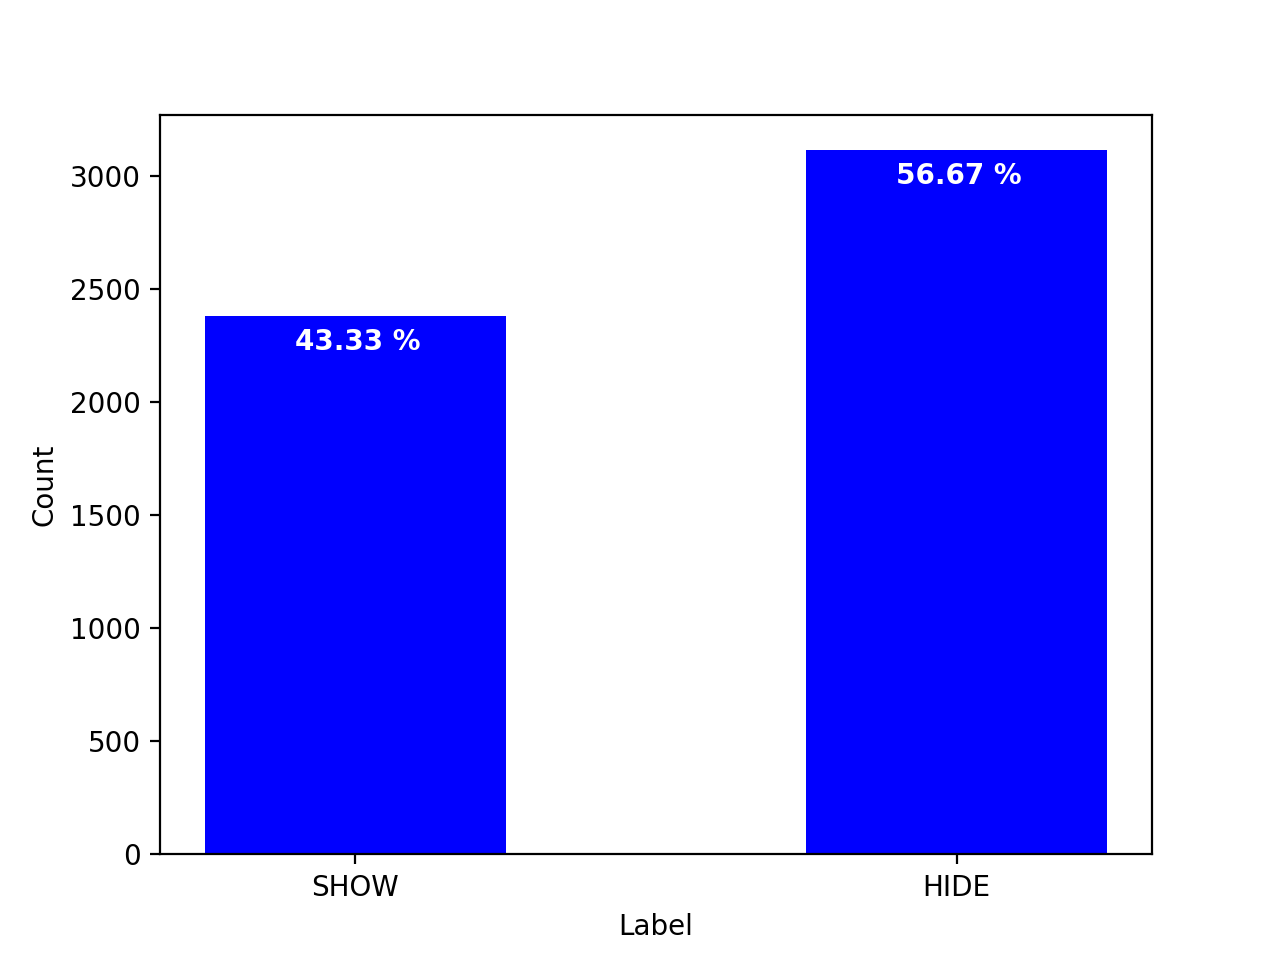
\includegraphics[width=\textwidth]{graphics/labels-dist}
			\end{subfigure}
			\hfill
			\begin{subfigure}{.4\textwidth}
				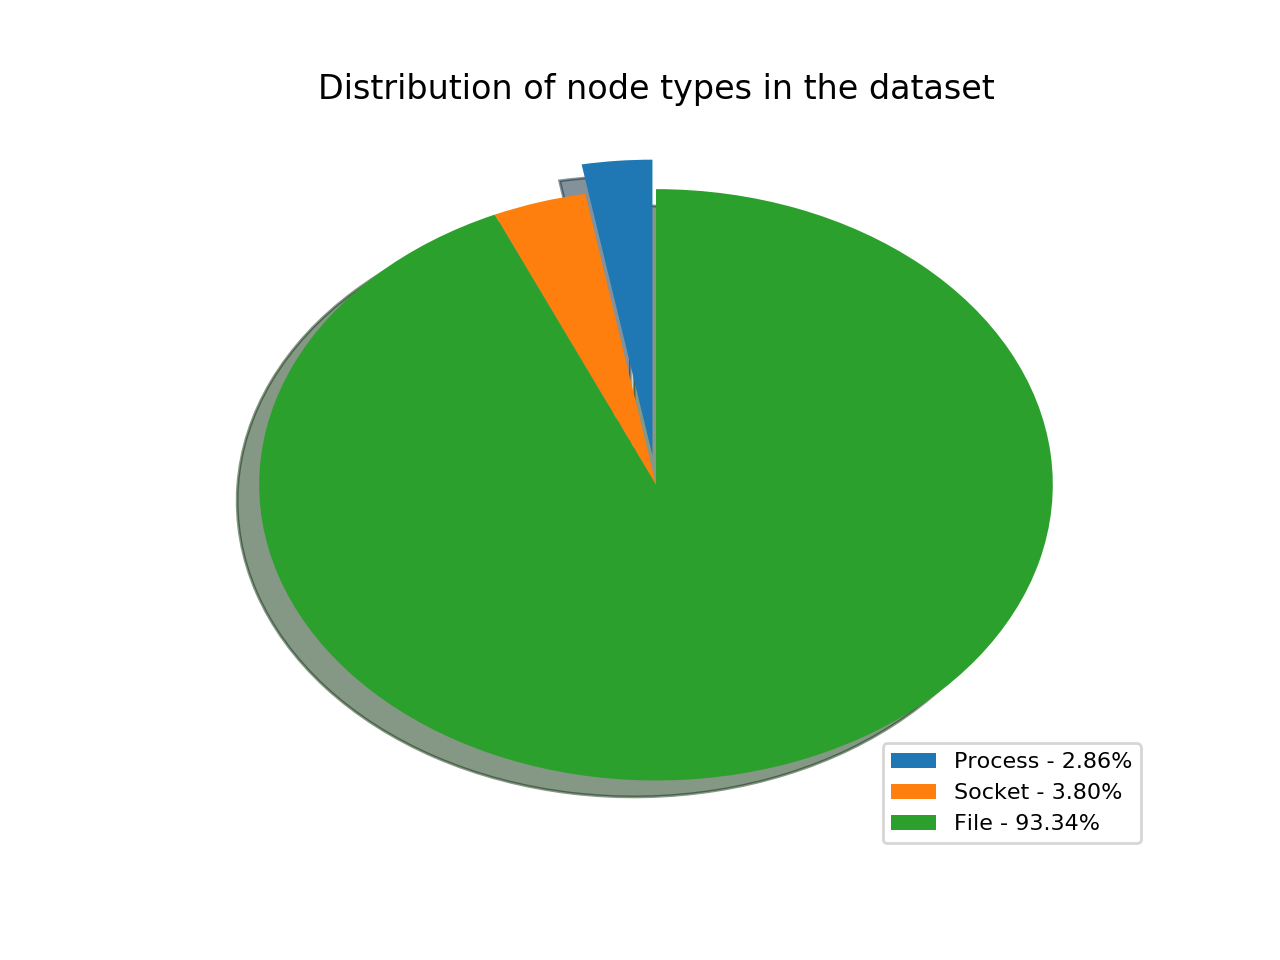
\includegraphics[width=\textwidth]{graphics/node-dist}
			\end{subfigure}
			\caption[Distributions of labels and node type in the dataset]{\textit{Left:} Distribution of the labels in the dataset. \textit{Right: }Distribution of the node types in the dataset.}
			\label{Fig: eval/ml/methodology/dist}
		\end{figure} 
		The technique used when evaluating the models was \textbf{k-fold cross validation}. Essentially, I split the dataset in $10$ equally-sized slots and use one at a time as a test set, while the other $9$ serve as the training set for the model. Figure \ref{Fig: impl/ml/methodology/kfold/first} shows how the dataset is divided in the first iteration of the cross-validation algorithm. For the models that require a validation set for optimising hyperparameters, the training set is split again in $10$ slots of equal sizes and uses one at a time as a validation set. This way, I ensure that none of the models is not tested on previously-seen examples and therefore I correctly evaluate how well they generalize on the given data.
		\begin{figure}[H]
			\centering
			\includegraphics[width=.8\textwidth]{graphics/k-fold}
			\caption{First step in k-fold cross validation}
			\label{Fig: impl/ml/methodology/kfold/first}
		\end{figure}
		
		At every iteration, I compute a set of metrics that for estimating the model's performance and the final result for every metric in part is given by averaging over the values obtained. 
	\subsection{Metrics involved} \label{Section: eval/ml/metrics}
	
		In this section, I will outline the metrics used when evaluating the machine learning models. The choice of good metrics is essential when comparatively evaluating a number of machine learning models. The simplest metric for evaluating of classification algorithms is \textbf{accuracy}, and can be computed using the formula: 
		\\
		\begin{equation}
			acc = \frac{\text{no. of correctly predicted nodes}}{\text{total no. of predicted nodes}}
		\end{equation}
		\\
		Accuracy, however, is not efficient when it comes to imbalanced data, as it is the case here(i.e. we have a $43\%/57\%$ \textit{SHOW/HIDE} distribution amongst the nodes). Therefore, more complex metrics are required in order to correctly assess the performance of the models implemented. These metrics are based on the notions of \textit{true positives, true negatives, false positives and false negatives}, which can easily be illustrated using a confusion matrix, such as the one from Figure \ref{Fig: eval/ml/metrics/confusion-matrix}.
		\begin{figure}[H]
			\centering
			\includegraphics[width=.7\textwidth]{graphics/confusion-matrix}
			\caption{Confusion matrix for two-class classification}
			\label{Fig: eval/ml/metrics/confusion-matrix}
		\end{figure}
		The metrics I used to evaluate the general performance of the models are presented in Table \ref{Table: eval/ml/metrics/metrics}. From those, the F1 score and the MCC are the most meaningful for this case, as they ignore the fact that the data is not balanced. The F1 score gives a value in the interval $[0, 1]$, with $1$ representing perfect prediction, while the MCC gives a value between $[-1, 1]$, where $1$ represents perfect prediction, $0$ not better than random and $-1$ a total disagreement between the predicted and true labels.
		\begin{longtable}{|p{.15\textwidth}|p{.40\textwidth}|c|}
		   \textbf{Metric} & \textbf{Intuition} &\textbf{Formula} \\
			\hline
			\textit{Precision} & fraction of nodes correctly labelled as \textit{SHOW} in all nodes classified. & {$\centering \text{precision} = \frac{tp}{tp+fp}$} \\
			\hline 
			\textit{Recall} & fraction of \textit{SHOW} nodes correctly classified. & $\text{recall} = \frac{tp}{tp+fn}$ \\
			\hline
			\textit{F1 score} & takes into consideration both the precision and the recall of the model in order to assess its performance & $\text{F1} = 2\times\frac{\text{precision}\times\text{recall}}{\text{precision} + \text{recall}}$\\
			\hline 
			\textit{Matthew's Correlation Coefficient (MCC)} & takes into account true and false positives and negatives in order to provide a balanced metric for the model's performance & $MCC = \frac{tp\times tn - fp\times fn}{\sqrt{(tp+fp)\times(tp+fn)\times(tn+fp)\times(tn+fn)}}$\\
			\hline
			\caption{Machine learning evaluation metrics}
			\label{Table: eval/ml/metrics/metrics}
		\end{longtable}
		
		\subsection{Results \& discussion} \label{Section: eval/ml/results}
	
	
		\section{Service time evaluation} \label{Section: eval/service-time}
		This project is meant to be a full API that can be used 
\end{document}